In our scenario, we have to face the problem of image recognition. Due to the large dimension of the feature representation for each image as well as the size of training image, manual classification is hopeless. As we mentioned in Section \ref{sec:intro:over}, a recognition model is used to distinguish the objects from different categories automatically trained by supervised learning. In this section, we introduce the classifiers we used in this thesis.

\subsection{Binary Classification and Multi-class Classification}

In image recognition, we train a recognition model from a set of training images along with their labels provided. The labels are predefined in a category space. Thus, the task of image recognition is to classify each image as one predefined category. If there are only two categories, this recognition task is called binary classification. For the task recognizing the objects from more than two categories, the recognition task is called multi-class classification \cite{aytar2011tabula} \cite{krizhevsky2012imagenet}.  

Here, we give a formal definition of the scenario for binary and multi-class classification. Generally, we can decompose the multi-class learning task into a set of binary scenarios by training a binary classifier for each class, e.g. One-VS-Rest strategy (see figure \ref{fig:related:ovsa})\cite{rifkin2004defense} \cite{tsoumakas2006multi}.

The binary scenario for classification can be defined as follow: given a dataset from domain $\mathcal{X} \times \mathcal{Y}$ where $\mathcal{X}$ is the input feature representation and $\mathcal{Y}$ is the binary label set $\{1,-1\}$ (for some classifier, $\{1,0\}$ is also used). We usually use the label $1$ to denote the examples belong to one certain category and -1 to denote examples not belong to that category. 
We assume that the training image set $D_{train}=\{(x_i,y_i)\} \subset \mathcal{X} \times \mathcal{Y}$ and the test image set $D_{test}=\{(x^t_i,y^t_i)\}\subset \mathcal{X} \times \mathcal{Y}$ are given and separated from each other. Each pair $(x_i,y_i)$ denotes the input feature representation $x_i$ and its corresponding label $y_i$ for the $i$\textit{th} image in the both set. Our goal of the classification problem is to learn a decision function $f:\mathcal{X} \rightarrow \mathcal{Y}$ from the training set $D_{train}$ such that $f$ can achieve good performance on both $D_{train}$ and $D_{test}$. 

\begin{figure}
	\centering
	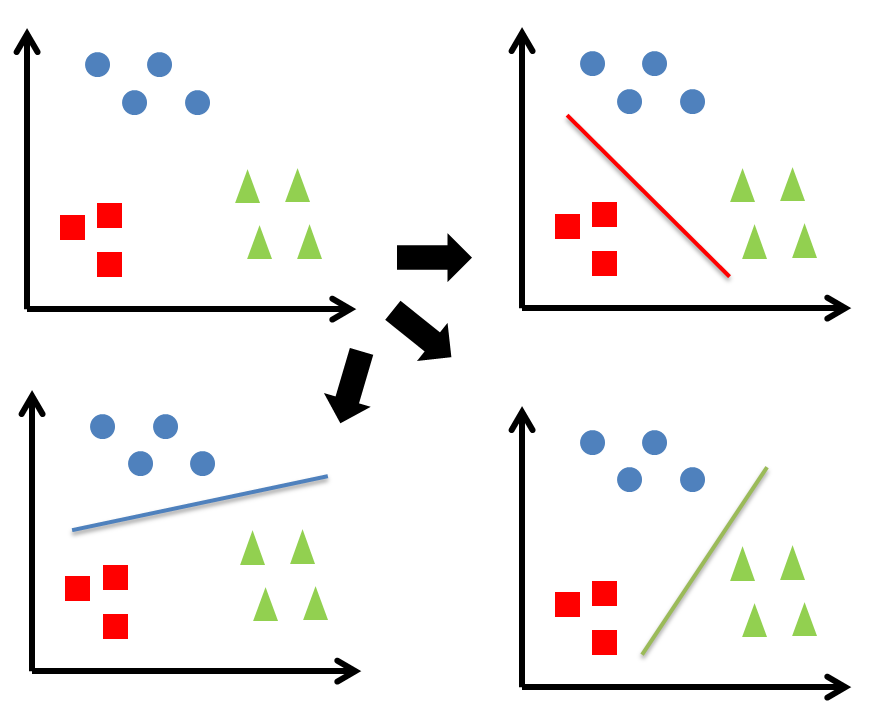
\includegraphics[scale=.8]{relatedwork/fig/ovsa.png}
	\caption{One-vs-Rest strategy for multi-class scenario. A three classes problem can be decomposed into 3 binary classification sub-problems.}\label{fig:related:ovsa}
\end{figure}
\subsection{Softmax Classifier}
In this subsection, we will introduce a widely used linear classifier \textbf{Softmax classifier} in image recognition. Linear classifier is commonly used as the classification model for image recognition. Linear classifier achieves this by making a classification decision based on the value of a linear combination of the input feature representations of a image. A linear classifier consists of two parts: a score function and a loss function. The score function maps the input data into the class scores and the loss function that quantifies the agreement between the predicted scores and the ground truth labels. Linear classifier often works very well when the number of dimensions of the input is large. Therefore, it is widely used as the classifier for image recognition, especially as the classifier for Convolutional Nueral Networks \cite{lecun1989backpropagation}. 

Typically, Softmax classifier is widely used for multi-class image classification.
Softmax classifier (also called multinomial logistic regression) is a generational form of logistic regression for the multi-class scenario. As logistic regression can only handle the binary classification scenario, Softmax classifier adapts the one-vs-rest strategy where several logistic regression models are trained for each class. 

Given a training set $\{(x_1,y_1),(x_2,y_2),...,(x_m,y_m)\}$, we assume the label $y_i \in \{1,0\}$ and the input feature $x_i \in \mathcal{R}^n$. For each binary logistic regression model, The score function takes the form:
\begin{equation}
	{f_w}(x) = \frac{1}{{1 + \exp ( - {w^T}x)}}
\end{equation}
and the parameters $w$ are optimized to minimize the following loss function:
\begin{equation}
	l(w) =  - [\sum\limits_{i = 1}^m {{y_i}\log {f_w}({x_i}) + (1 - {y_i})} \log (1 - {f_w}({x_i}))]\label{eq:logistic:loss}
\end{equation}

For Softmax classifier, it is used to handle the multi-class classification problem and suppose there are $N$ classes. Therefore, $y$ can take from $N$ different values $\{1,2,3,...,N\}$ instead of just two. For a given test example $x$, the score function estimate the probability $P(y=n|x)$ for each value of $n = 1,2,3,...,N$, i.e. estimate the probability that each score assigns the input $x$ to the $N$ classes associated to the $N$ different possible values. Thus, the score function will output a $N$-dimensional vector providing $N$ estimated probabilities whose sum of elements is 1. The $N$ dimensional output of the score function can be generated according to the following form:
\begin{equation}
{f_w}\left( x \right) = \left[ \begin{array}{l}
P\left( {y = 1|x;w} \right)\\
P\left( {y = 2|x;w} \right)\\
...\\
P\left( {y = n|x;w} \right)
\end{array} \right] = \frac{1}{{\sum\nolimits_{j = 1}^N {\exp \left( {{w^{(j)T}}x} \right)} }}\left[ \begin{array}{l}
\exp \left( {{w^{(1)T}}x} \right)\\
\exp \left( {{w^{(2)T}}x} \right)\\
...\\
\exp \left( {{w^{(N)T}}x} \right)
\end{array} \right]
\end{equation}
Here $w^{(1)T},w^{({2})T},...,w^{({N})T}$ are the parameters of the Softmax classifier model. The term $\frac{1}{{\sum\nolimits_{j = 1}^N {\exp \left( {{w^{(j)T}}x} \right)} }}$ is called the normalization term so that the $N$ distributions sum to 1.

To optimize the parameters $w^{(1)T},w^{({2})T},...,w^{({N})T}$, the cross-entropy loss used for the Softmax classifier is defined as:
\begin{equation}
J(w) =  - \left[ {\sum\limits_{i = 1}^l {\sum\limits_{k = 1}^N {\ell\left\{ {{y_i} = k} \right\}\log \frac{{\exp \left( {{w^{(k)T}}x_i} \right)}}{{\sum\nolimits_{j = 1}^N {\exp \left( {{w^{(j)T}}x_i} \right)} }}} } } \right] \label{eq:softmax:loss}
\end{equation}
Here $\ell{x}$ is the 0-1 loss function:
\begin{equation}
\ell \{ x\}  = \left\{ {\begin{array}{*{20}{c}}
	1&\text{$x$ is true}\\
	0&\text{$x$ is false}
	\end{array}} \right. 
\end{equation}
It is noted that Eq \eqref{eq:softmax:loss} is a generalized form of Eq \eqref{eq:logistic:loss}. Minimizing Eq \eqref{eq:softmax:loss} can be interpreted as minimizing the negative log likelihood of the correct class, which is equivalent to performing Maximum Likelihood Estimation (MLE) \cite{johansen1990maximum}.

The minimum of $J(w)$ can be obtained by gradient descent method while taking the gradient:
\begin{equation}
\nabla J({w^{(n)}}) =  - \sum\limits_{i = 1}^l {\left[ {{x_i}\left( {\ell \left\{ {{y_i} = n} \right\} - \frac{{\exp \left( {{w^{(k)T}}x_i} \right)}}{{\sum\nolimits_{j = 1}^N {\exp \left( {{w^{(j)T}}x_i} \right)} }}} \right)} \right]} 
\end{equation}

\subsection{Support Vector Machines}
In this subsection, we will review another widely used discriminant classifier, \textbf{Support Vector Machine} (SVM) \cite{cristianini2000introduction}. SVM is another classifier that has been adoptive in many image recognition tasks \cite{coates2011analysis} \cite{schuldt2004recognizing} \cite{yang2009linear}. In this thesis, we also use a classifier based on SVM. We will give a detailed description of SVM. 

As we mentioned before, the linear classifier consists of two parts: the score function and loss function. SVM classifier can be divided into two categories based on their score function: linear SVM that uses a linear discriminant function and kernel SVM that uses kernel function. Kernel SVM can be considered as a extension version of linear SVM where kernels are used for calculate the scores of the inputs. Another difference for between linear and kernel SVM is linear SVM can be solved on the primal problem while kernel SVM is mostly optimized on its dual \cite{cristianini2000introduction} \cite{shalev2011pegasos}.

First, we will introduce the linear SVM. Linear SVM uses the simplest representation of a score function by taking the linear combination of the input vector:
\begin{equation}\label{eq:relation:score}
f(x) = w^Tx+b
\end{equation}
where $w$ is called the weight vector and $b$ is called the bias. In a binary scenario, for the input example $x$ and the class labels $y \in \{c1,c2\}$, $x$ is assigned to class $c1$ if $f(x) \geq 0$ and $c2$  otherwise. Therefore, the corresponding decision surface is defined by $f(x)=0$. For two points $x_1$ and $x_2$ lie on the decision surface, we have $f(x_1)=f(x_2)=0$. Then we can have $w^T(x_1-x_2)=0$ and hence the weight vector $w$ is orthogonal to every point lying within the decision surface, i.e $w$ determines the orientation of the decision surface. Similarly, if $x$ lies on the decision surface, the normal distance from the origin to the decision surface is given by:
\begin{equation}
\frac{w^Tx}{||w||}=-\frac{b}{||w||}
\end{equation}
Therefore, we can see that, the location of the decision surface is determined by the bias $b$.
\subsubsection{Hard Margin SVM}
Hard margin SVM is used to find the optimal solution for the data sets that are linear separable. 
Given a set of n training points $(x_1,y_1),(x_2,y_2),...,(x_n,y_n)$ where $y_i \in \{1,-1\}$, we expect to find a decision surface that can separate the data from two classes. However, when the data from these two classes can be linearly separated, there could be several decision surfaces that can separate the data. The idea of SVM is to choose the maximal margin decision surface so that the distance between these two classes is as large as possible (called maximal margin hyperplane). For example, in figure \ref{fig:relate:svm}\subref{fig:relate:svma}, $H2$ and $H3$ are two candidate decision surface that can separate the data. However, $H3$ is has the largest distance to all the data from two classes and SVM will choose $H3$ as the optimal hyperplane. 

\begin{figure}
	\centering
	\subfloat[Different sparating hyperplanes]{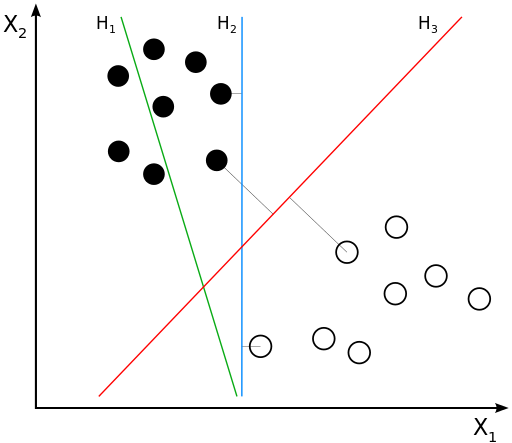
\includegraphics[width = 0.45\textwidth]{relatedwork/fig/svm2.png}\label{fig:relate:svma}}
	\subfloat[Max-Margin hyperplanes]{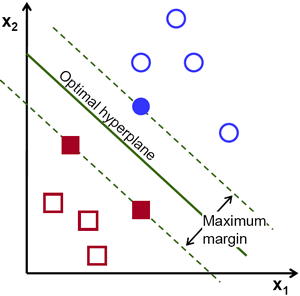
\includegraphics[width = 0.4\textwidth]{relatedwork/fig/svm1.png}}
	\caption{Support Vector Machine}\label{fig:relate:svm}
\end{figure}
The optimal hyperplane can be found by minimizing the following objective function:
\begin{equation}
\begin{aligned}
\min \qquad & ||w||^2\\
\text{s.t.}\qquad & y_i(w^Tx_i+b) \geq 1 \quad \text{for all } 1\leq i \leq n
\end{aligned}
\end{equation}
\subsubsection{Soft Margin SVM}
In real world application, most data are not linear separable. Therefore, SVM introduce the concept of slack variable to handle this situation. Slack variable is defined as:
\begin{equation}
\xi_i  = hinge(x_i) = \max (0,1-y_i(w^Tx_i+b))
\end{equation}
The value of slack variable is 0 if the example $x_i$ lies on the correct side of the margin. For those data on the wrong side, its value is proportional to the distance from the correct margin.
\begin{figure}
	\centering
	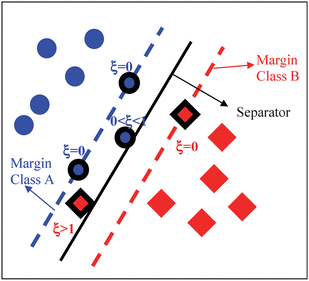
\includegraphics[scale =1.2]{relatedwork/fig/slack.png}
	\caption{Slack variables for soft-margin SVM}
\end{figure}

Therefore, to find the parameters of hyperplane, i.e. weight vector $w$ and bias $b$, soft-margin SVM minimize the following loss function:
\begin{equation}\label{eq:related:softsvm}
	\begin{aligned}
	\min \qquad &  \frac{\lambda}{2}||w||^2+\frac{1}{n}\sum_{i}^{n}\xi_i\\
	\text{s.t.}\qquad & y_i(w^Tx_i+b) \geq 1-\xi_i \\
	& \xi_i \geq 0 	\quad \text{for all } 1\leq i \leq n
	\end{aligned}
\end{equation}
The objective function is called primal of SVM. A stochastic sub-gradient descent can be used to find the optimal solution for eq. \eqref{eq:related:softsvm} effectively \cite{shalev2011pegasos}. 
\subsubsection{Kernel SVM}
Linear soft-margin SVM works well when number of features is larger than number of training examples. However, when the size of the training example is larger than the features, kernel SVM (such as Gaussian Kernel) with proper parameters outperforms linear SVM \cite{keerthi2003asymptotic}.
\begin{figure}
	\centering
	{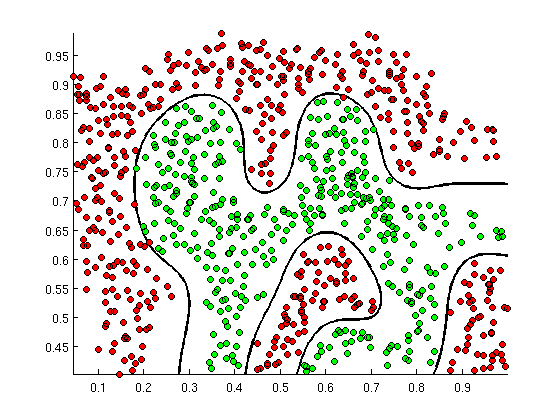
\includegraphics[width = 0.8\textwidth]{relatedwork/fig/non-linear2.png}}
	\caption{The hyperplane of SVM with RBF kernel for non-linear separable data.}\label{fig:relate:nonlinear}
\end{figure}

The idea of kernel was first introduced into pattern recognition by Aizerman \textit{et. al.} \cite{aizerman1964probability}. When the size of the training examples are significantly larger than the dimension of the input features and the distribution become more complex, these data can not be easily separated by a straight line in the feature space.
Instead of obtaining the optimal hyperspace in the input feature space, kernel SVM tries to map the inputs into a high-dimensional feature spaces and find the optimal hyperplane in the high-dimensional feature spaces. Given a feature space mapping $\phi(x)$, the score function for kernel SVM can be re-written as:
\begin{equation}\label{eq:relation:kernel}
	f(x) = w^T\phi(x)+b
\end{equation}
From eq \eqref{eq:relation:kernel} we can see that, when we take the identity mapping $\phi(x) = x$, the kernel SVM becomes a linear SVM. Therefore, the linear SVM can be considered as a special case of kernel SVM where identity mapping is used as the kernel. The loss function of kernel SVM is almost identical to eq. \eqref{eq:related:softsvm} except for replacing the term $x$ with $\phi(x)$: 
\begin{equation}\label{eq:related:primal}
\begin{aligned}
\min \qquad &  \frac{\lambda}{2}||w||^2+\frac{1}{n}\sum_{i}^{n}\xi_i\\
\text{s.t.}\qquad & y_i(w^T\phi(x)_i+b) \geq 1-\xi_i \quad \\
& \xi_i \geq 0 	\quad \text{for all } 1\leq i \leq n
\end{aligned}
\end{equation}
By introducing the Lagrangian term to the primal \eqref{eq:related:primal} and some transformation, we obtain the dual of kernel SVM function:
\begin{equation} \label{eq:related:dual}
	\begin{aligned}
	\max \qquad& \sum_{i}^{n}\alpha_i-\sum\limits_i^n {\sum\limits_j^n {{y_i}{y_j}{\alpha _i}} } {\alpha _j}\phi ({x_i})\phi ({x_j})\\
	\text{s.t.} \qquad & 0 \leq \alpha_i \leq \frac{1}{\lambda}\\
	& \sum_{i}^{n}y_i\alpha_i=0 \quad \text{for all } 1\leq i \leq n
	\end{aligned}
\end{equation}
We can obtain the solution of \eqref{eq:related:dual} by Sequential Minimal Optimization (SMO) \cite{platt1998sequential} or Dual Coordinate Descent \cite{hsieh2008dual}.

There are several advantages of using SVM as the classifier: 
\begin{itemize}
	\item \textbf{Generalization ability.} SVM provides good generalization ability by maximizing the margin between the examples of the two classes. By setting the proper parameters and generalization grade, SVM can overcome some bias from the training set. Therefore, SVM is able to make correct prediction for unseen data. This ability can be very useful for image recognition as there is no image dataset that can cover all the transformation of the objects. Moreover,the idea of soft-margin makes it robust against noisy data.
	\item \textbf{Kernel transformation.} By introducing the non-linear transformation of the input, SVM can model complex non-linear distributed data. The kernel trick can greatly improve the computational efficiency.   
	\item \textbf{Unique solution.} The objective function of SVM is  convex. Compared to other methods, such as Neural Networks, which are non-convex and have many local minima, SVM can deliver a unique solution for any given training set and can be solved with efficient methods, like sub-SGD \cite{shalev2011pegasos} or SMO \cite{platt1998sequential}. 
\end{itemize}

